\documentclass[aspectratio=169]{beamer}

\usetheme{Madrid}
\usecolortheme{default}
\usepackage[T1]{fontenc}
\usepackage[utf8]{inputenc}
\usepackage{lmodern}
\usepackage{booktabs}
\usepackage{array}
\usepackage{graphicx}
\usepackage{hyperref}
\usepackage{tikz}
\usetikzlibrary{shapes.arrows, positioning}

\title[Applied Project — Football Analysis]{Real-time Football Match Analysis:\\From Raw Video to Tactical Insights}
\author{Alessandro ARENSBERG}
\institute{Albert School}
\date{May 19, 2026}

\newcommand{\placeholderfigure}[1]{%
  \fbox{\parbox[c][3.2cm][c]{0.96\linewidth}{\centering \textit{#1}}}%
}

\begin{document}

\begin{frame}
  \titlepage
\end{frame}

\section{The Challenge}
\begin{frame}{The Challenge: Understanding Football in Real Time}
  \vspace{-0.3cm}
  \begin{center}
    \textbf{Watch a 30-second broadcast clip. What does the camera see?}
  \end{center}
  
  \vspace{0.3cm}
  \begin{itemize}
    \item \textbf{22 players} moving at different speeds
    \item \textbf{2 referees} on the pitch
    \item \textbf{1 ball} (very small, frequently occluded)
    \item \textbf{Camera motion} following the action
    \item \textbf{Compression, blur, lighting changes}
  \end{itemize}

  \vspace{0.4cm}
  \textit{Now ask a machine to find all of this, track everyone consistently, and output match statistics.}
  
  \vspace{0.2cm}
  This is \textbf{not} trivial—especially for small objects under occlusion and camera motion.
\end{frame}

\section{Why This Matters}
\begin{frame}{The Real-World Problem}
  \begin{columns}[T]
    \column{0.48\textwidth}
    \textbf{Use cases:}
    \begin{itemize}
      \small
      \item Coaching: tactical analysis
      \item Scouting: player evaluation
      \item Analytics: possession, heat maps
    \end{itemize}
    
    \column{0.48\textwidth}
    \textbf{The bottleneck:}
    \begin{itemize}
      \small
      \item Manual annotation is slow
      \item Broadcasting needs real-time output
      \item Volume is massive (thousands of matches/year)
    \end{itemize}
  \end{columns}
  
  \vspace{0.4cm}
  \textit{We need automation that actually works.}
\end{frame}

\section{Solution}
\begin{frame}{The Pipeline: A Multi-Stage Approach}
  \centering
  \vspace{-0.3cm}
  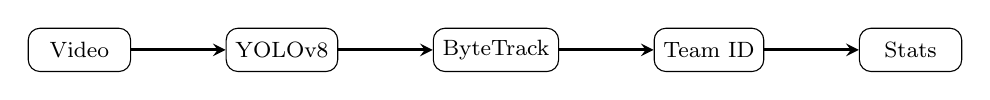
\begin{tikzpicture}[
    node distance=1.2cm,
    every node/.style={
      draw,
      rectangle,
      rounded corners=0.15cm,
      minimum width=1.3cm,
      minimum height=0.55cm,
      font=\footnotesize,
      align=center
    },
    every edge/.style={draw, thick, -stealth, line width=1pt}
  ]
    \node (video) {Video};
    \node (yolo) [right=of video] {YOLOv8};
    \node (track) [right=of yolo] {ByteTrack};
    \node (team) [right=of track] {Team ID};
    \node (stats) [right=of team] {Stats};
    
    \draw (video) edge (yolo)
          (yolo) edge (track)
          (track) edge (team)
          (team) edge (stats);
  \end{tikzpicture}
  
  \vspace{0.5cm}
  \small
  \begin{itemize}
    \item \textbf{Detection:} Fine-tuned YOLOv8 on football videos
    \item \textbf{Tracking:} Persistent IDs + memory for fragmentation
    \item \textbf{Recovery:} Ball interpolation, ROI search, optical flow
    \item \textbf{Team Assignment:} Jersey colour clustering
    \item \textbf{Output:} Speed, distances, possession, formation lines
  \end{itemize}
\end{frame}

\begin{frame}{Key Technical Insight}
  \textbf{Naive approach:} Train a big detector, run inference. \textit{Result: fragmented tracks, poor ball coverage.}
  
  \vspace{0.3cm}
  \textbf{Our approach:} Detection + \textbf{temporal reasoning}
  \begin{itemize}
    \item Ball interpolation: Fill gaps $\le 6$ frames
    \item Track memory: Reactivate IDs on IoU > 0.2
    \item Team freezing: Prevent mid-possession flips
    \item Camera compensation: Stabilize position drift
  \end{itemize}

  \vspace{0.3cm}
  \textit{Lesson: Post-processing matters as much as the detector.}
\end{frame}

\section{Results}
\begin{frame}{Baseline vs Fine-Tuned: The Impact of Domain Knowledge}
  \centering
  \small
  \begin{table}
    \begin{tabular}{llrrrr}
      \toprule
      \textbf{Model} & \textbf{Ball Frames} & \textbf{Player Tracks} & \textbf{Referees} & \textbf{Stability} \\
      \midrule
      Generic YOLOv8n & 736/750 (98\%) & 22,530 & \textbf{0} & Fragmented \\
      Fine-tuned YOLOv8 & 715/750 (95\%) & 15,488 & \textbf{2,118} & Stable \\
      \bottomrule
    \end{tabular}
  \end{table}
  
  \vspace{0.3cm}
  \textbf{Counterintuitive:} Generic model sees \textit{more} ball frames but has 31\% more fragmentation.
  
  \vspace{0.2cm}
  \textit{More detections $\neq$ better tracking. Quality beats quantity.}
\end{frame}

\begin{frame}{What Fine-Tuning Achieved}
  \begin{itemize}
    \item \textbf{\textcolor{green}{+}} Referee detection: \textbf{0} $\to$ \textbf{2,118 frames}
      \begin{itemize}
        \small
        \item Generic model completely misses referees
        \item Critical for tactical analysis
      \end{itemize}
    
    \vspace{0.2cm}
    \item \textbf{\textcolor{green}{+}} Reduced fragmentation: \textbf{22,530} $\to$ \textbf{15,488 tracks (−31\%)}
      \begin{itemize}
        \small
        \item Fewer identity switches = better downstream stats
      \end{itemize}
    
    \vspace{0.2cm}
    \item \textbf{\textcolor{green}{+}} Team stability
      \begin{itemize}
        \small
        \item Generic: 78 + 110 fragmented identities
        \item Fine-tuned: 17 + 33 stable identities
      \end{itemize}
  \end{itemize}
\end{frame}

\begin{frame}{Ablation: What Component Matters Most?}
  \centering
  \small
  \begin{table}
    \begin{tabular}{lrr}
      \toprule
      \textbf{Variant} & \textbf{Ball Frames} & \textbf{Loss} \\
      \midrule
      Full pipeline & 715/750 (95.3\%) & — \\
      No interpolation & 664/750 (88.5\%) & −51 frames (−6.8\%) \\
      No track memory & 700/750 (93.3\%) & −15 frames (−2.0\%) \\
      \bottomrule
    \end{tabular}
  \end{table}
  
  \vspace{0.3cm}
  \textbf{Key finding:} Ball interpolation is the biggest driver.
  
  \vspace{0.2cm}
  \textit{Temporal priors are crucial for small-object tracking.}
\end{frame}

\section{Failures}
\begin{frame}{Where It Fails: The Hard Cases}
  \begin{columns}[T]
    \column{0.48\textwidth}
    \textbf{Goalkeeper ambiguity}
    \begin{itemize}
      \small
      \item Detector oscillates between "player" and "goalkeeper"
      \item Early-game keepers often undetected
      \item Visual similarity makes classification hard
    \end{itemize}
    
    \column{0.48\textwidth}
    \textbf{Ball challenges}
    \begin{itemize}
      \small
      \item Motion blur on fast kicks
      \item Aerial balls merge with crowd
      \item Out-of-frame recovery fails
    \end{itemize}
  \end{columns}
  
  \vspace{0.3cm}
  \begin{columns}[T]
    \column{0.48\textwidth}
    \textbf{Tracking}
    \begin{itemize}
      \small
      \item Camera pans $\to$ position jitter
      \item Dense occlusions $\to$ ID switches
    \end{itemize}
    
    \column{0.48\textwidth}
    \textbf{Metric conversion}
    \begin{itemize}
      \small
      \item No ground-truth calibration
      \item Speed estimates: $\pm 20\%$ error
    \end{itemize}
  \end{columns}
\end{frame}

\begin{frame}{Root Cause Analysis}
  \begin{itemize}
    \item \textbf{Goalkeeper issue:} Classifier confusion, not just post-processing
      \begin{itemize}
        \small
        \item Mitigation: Field position heuristics, ensemble voting
        \item Real fix: Collect more goalkeeper training data
      \end{itemize}
    
    \vspace{0.2cm}
    \item \textbf{Ball tracking:} Physics missing from detector
      \begin{itemize}
        \small
        \item Mitigation: Interpolation, ROI search
        \item Real fix: Temporal CNN or Kalman filter with physics
      \end{itemize}
    
    \vspace{0.2cm}
    \item \textbf{Calibration:} No reference points in broadcast video
      \begin{itemize}
        \small
        \item Mitigation: Approximate scaling (105m $\times$ 68m)
        \item Real fix: Line detection or manual homography
      \end{itemize}
  \end{itemize}

  \vspace{0.2cm}
  \textit{Not all problems are solvable at the detector level.}
\end{frame}

\section{Conclusion}
\begin{frame}{Key Learnings}
  \begin{enumerate}
    \item \textbf{Domain knowledge wins:} Football-specific fine-tuning beats generic baseline
    
    \vspace{0.15cm}
    \item \textbf{Temporal reasoning is essential:} Tracking + interpolation $>$ detection alone
    
    \vspace{0.15cm}
    \item \textbf{Post-processing is underrated:} Team freezing, memory, recovery stabilize output
    
    \vspace{0.15cm}
    \item \textbf{Failure analysis reveals gaps:} Not every problem is solvable with bigger models
  \end{enumerate}
  
  \vspace{0.35cm}
  \textbf{Bottom line:} A careful multi-stage pipeline outperforms naive end-to-end approaches.
\end{frame}

\begin{frame}{What's Next?}
  \begin{itemize}
    \item Real-time deployment (edge optimization for streaming)
    \item Multi-view tracking (integrate stadium camera feeds)
    \item Tactical event detection (passes, shots, fouls, set pieces)
    \item Interactive labeling (active learning loop)
  \end{itemize}
  
  \vspace{0.3cm}
  \textit{The core system works. Now we scale and specialize it.}
\end{frame}

\begin{frame}
  \centering
  \Large
  \textbf{Thank You}
  \vspace{0.6cm}
  
  \\
  \normalsize
  Questions?
  
  \vspace{0.4cm}
  {\small Output: \texttt{output/08fd33\_4-colab\_v3\_51e\_1920\_b2-best-...mp4}}
\end{frame}

\end{document}